\documentclass[12pt,a4paper]{article}

\usepackage[utf8]{inputenc}
\usepackage{amsmath, amssymb}
\usepackage{graphicx}
\usepackage{geometry}
\usepackage{hyperref}
\usepackage{lipsum}
\usepackage[numbers, square, comma]{natbib}
\usepackage{tikz}
\usepackage{appendix}
\usepackage{cleveref}

\crefname{figure}{Figure}{Figures}
\crefname{equation}{Equation}{Equations}
\geometry{margin=1in}

\title{Euler's Formula: Connecting Exponentials and Trigonometry}
\author{Eckhardt Alvarez Ian}
\date{\today}

\begin{document}
\maketitle
\tableofcontents

\section{Introduction}
Euler's formula is one of the most important formulas in complex analysis; it establishes a connection between complex exponential functions and trigonometric functions. Euler's formula states that for any real number $\theta$:
\begin{equation}
e^{i\theta} = \cos{\theta} + i\sin{\theta}.
\end{equation}
This formula is an elegant way of connecting seemingly unrelated areas in mathematics: complex numbers with the use of the imaginary unit $i$, exponentials and the number $e$ (the base of the natural logarithm), and trigonometry with the sine and cosine functions that describe circular motion.
Euler's formula is important because of its use in various areas in mathematics, such as complex analysis, topology, Fourier analysis, and quaternions, making this formula a fundamental one to understand.
\pagebreak
\section{Understanding and Deriving Euler's formula}
\subsection{Understanding the formula}
To understand how Euler's formula works, we first examine its components. The first component we see is the exponential function $e^x$, defined as:
\begin{equation}
e^x = \lim_{n\to\infty} \left(1 + \frac{x}{n}\right)^n.
\end{equation}
Euler's formula uses $e^{i\theta}$, which by this definition we could write as
\(
\lim_{n\to\infty} \left(1 + \frac{i\theta}{n}\right)^n
\).
The next element of Euler's formula we see is $i$, the imaginary unit defined as the solution to the equation $x^2+1=0$, where $i = \sqrt{-1}$ (note that $-i$ is also a solution). $i$ can be used to extend the real numbers to what are called complex numbers. 

Imaginary numbers are an important mathematical concept; not only do they extend the real number system $\mathbb{R}$ to the complex number system $\mathbb{C}$, but also can be interpreted geometrically as rotations on the complex plane, such as a $\theta$-radian rotation by exponentiating by $i\theta$, or a $90^{\circ}$ rotation by multiplying by $i$ (this occurs because $i = e^{i\frac{\pi}{2}}$, which represents a counterclockwise rotation by $\frac{\pi}{2}$ radians; this is derived in Appendix~\ref{app:AppendixC}).

The last elements of the equation are the trigonometric functions $\sin{\theta}$ and $\cos{\theta}$; these functions can be defined using a right-angled triangle based on the angle of interest as:
\begin{align}
\sin{\theta} &= \frac{\text{opposite}}{\text{hypotenuse}}, & \cos{\theta} = \frac{\text{adjacent}}{\text{hypotenuse}}
\end{align}
These functions can also be defined in terms of exponentials as:
\begin{align}
\sin{\theta} &= \frac{e^{i\theta}-e^{-i\theta}}{2i}, & \cos{\theta} = \frac{e^{i\theta}+e^{-i\theta}}{2}.
\end{align}
These definitions are derived by solving for $\sin{\theta}$ and $\cos{\theta}$ using Euler's formula, for the derivation see Appendix~\ref{app:AppendixA}. Geometrically, Euler's formula can be seen in a unit circle in the complex plane like this:
\begin{figure}[ht]
\begin{center}
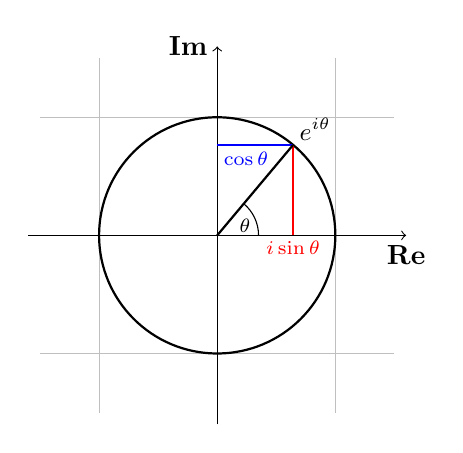
\begin{tikzpicture}[scale=1.5pt]
\draw[very thin,gray!50] (-1.5,-1.5) grid (1.5,1.5);
\draw[->] (-1.6,0) -- (1.6,0) node[anchor=north] {\textbf{Re}};
\draw[->] (0,-1.6) -- (0,1.6) node[anchor=east] {\textbf{Im}};
\draw[thick] (0,0) circle (1);
\draw(0.35,0) arc (0:50:0.35) node[left, xshift=6pt, yshift=-8pt] {\scriptsize{$\theta$}};
\draw[-, thick, blue] (0,0.766) -- (0.6427,0.766) node[xshift=-17pt, yshift=-5pt] {\scriptsize{$\cos{\theta}$}};
\draw[-, thick, red] (0.6427,0) -- (0.6427,0.766) node[below, yshift=-31pt] {\scriptsize{$i\sin{\theta}$}};
\draw[-, thick] (0,0) -- (0.6427,0.766) node[above, xshift=8pt, yshift=-2pt] {\small{$e^{i\theta}$}};
\end{tikzpicture}
\end{center}\caption{\textit{Unit Circle in the complex plane.} The complex number $e^{i\theta}$ plotted on the unit circle, with $\cos{\theta}$ on the real axis and $i\sin{\theta}$ on the imaginary axis.}\label{fig:UnitCircle}
\end{figure}\\
As seen on~\cref{fig:UnitCircle}, the complex number $e^{i\theta}$ is a composition of the $\cos{\theta}$ on the real axis and $i\sin{\theta}$ placing the sine on the imaginary axis, representing $e^{i\theta}$ as a point on the complex plane using trigonometric functions.

\subsection{Deriving the formula}
There are many formulas to derive Euler's equation, but the one we are going to use in this paper is with the help of the Taylor series to approximate a function into an infinite polynomial around a point (explained with more detail on Appendix~\ref{app:AppendixB}), the Taylor series of a function $f(x)$ around a point $a$ is:
\begin{equation}
f(x) = \sum_{n = 0}^\infty \frac{\left.\frac{d^{n}f}{dx^n}\right|_{x=a}}{n!}(x - a)^n
\end{equation}
Using the Taylor series will help us to convert sine and cosine into polynomials:
\begin{align}
\sin{\theta}  &= \sum_{n = 0}^\infty \frac{\left.\frac{d^{n}\sin{\theta}}{d\theta^n}\right|_{\theta=0}}{n!}\theta^n\nonumber\\
&= \sum_{n=0}^\infty \frac{(-1)^n}{(2n + 1)!}\theta^{2n + 1}\\
&= \theta - \frac{\theta^3}{3!} + \frac{\theta^5}{5!} - \frac{\theta^7}{7!} + \cdots\\\nonumber\\
\cos{\theta} &= \sum_{n = 0}^\infty \frac{\left.\frac{d^{n}\cos{\theta}}{d\theta^n}\right|_{\theta=0}}{n!}\theta^n\nonumber\\
&= \sum_{n=0}^\infty \frac{(-1)^n}{(2n)!}\theta^{2n}\\
&= 1 - \frac{\theta^2}{2!} + \frac{\theta^4}{4!} - \frac{\theta^6}{6!} + \cdots
\end{align}
Doing the same for \(e^{i\theta}\) gives us:
\begin{align}
e^{i\theta} &=  \sum_{n = 0}^\infty \frac{\left.\frac{d^n e^{i\theta}}{d\theta^n}\right|_{\theta=0}}{n!}\theta^n\nonumber
\end{align}
Since $\frac{d^n}{d\theta^n}e^{i\theta} = i^ne^{i\theta}$, evaluated at $\theta = 0$, we have $\left.\frac{d^{n}e^{i\theta}}{d\theta^n}\right|_{\theta=0} = i^n$.
\begin{align}
e^{i\theta} &= \sum_{n = 0}^\infty i^n\frac{\theta^n}{n!}\\
&= \frac{\theta^0}{1} + i\frac{\theta}{1!} + i^2\frac{\theta^2}{2!} + i^3\frac{\theta^3}{3!} + i^4\frac{\theta^4}{4!} + i^5\frac{\theta^5}{5!} + i^6\frac{\theta^6}{6!}\cdots\nonumber\\
&=  1 + i\theta - \frac{\theta^2}{2} - i\frac{\theta^3}{3!} + \frac{\theta^4}{4!} + i\frac{\theta^5}{5!} - \frac{\theta^6}{6!}\cdots\nonumber\\
&= \left(1 - \frac{\theta^2}{2!} + \frac{\theta^4}{4!} - \frac{\theta^6}{6!} + \cdots\right) + i\left(\theta - \frac{\theta^3}{3!} + \frac{\theta^5}{5!} - \cdots\right)
\end{align}
As we see, the Taylor series of $e^{i\theta}$ is just the sum of the Taylor series of $\cos{\theta}$ and the Taylor series of $\sin{\theta}$ multiplied by $i$, thus:
\[
e^{i\theta} = \cos{\theta} + i\sin{\theta},
\]
connecting exponentials and trigonometric functions in an elegant way.

\section{Conclusion}
As we have seen along this paper, Euler's formula is an impactful formula that is able to connect exponentials and trigonometric functions with the help of imaginary numbers; this connection leads to various advancements in diverse areas of math and science, with its applications spanning signal processing, electrical engineering, topology, and even quantum mechanics. Euler's formula exemplifies the unity of all mathematical fields in both abstract and physical ways.

\appendix
\crefalias{section}{appsec}
\section{Deriving Sine and Cosine Using Euler’s Formula}\label{app:AppendixA}
We will start with the derivation for $\sin{\theta}$, starting with Euler's formula:
\begin{align*}
e^{i\theta} &= \cos{\theta} + i\sin{\theta}\\
e^{-i\theta} &= \cos{-\theta} + i\sin{-\theta}
\end{align*}
Since $\cos{\theta}$ is an even function (meaning $f(-x) =f(x)$) and $\sin{\theta}$ is an odd function (meaning $f(-x) = -f(x)$) we get
\[
e^{-i\theta} = \cos{\theta} - i\sin{\theta}
\]
To isolate $\sin{\theta}$, subtract $e^{-i\theta}$ from $e^{i\theta}$ we get:
\begin{align*}
e^{i\theta} - e^{-i\theta} &= \cos{\theta} + i\sin{\theta} - (\cos{\theta} - i\sin{\theta})\\
&= \cos{\theta} + i\sin{\theta} - \cos{\theta} + i\sin{\theta}\\
&= 2i\sin{\theta}\\
\frac{e^{i\theta} - e^{-i\theta}}{2i} &= \sin{\theta}
\end{align*}
To isolate $\cos{\theta}$, add $e^{-i\theta}$ from $e^{i\theta}$ instead of subtracting, giving us:
\begin{align*}
e^{i\theta} + e^{-i\theta} &= \cos{\theta} + i\sin{\theta} + \cos{\theta} - i\sin{\theta}\\
&= 2\cos{\theta}\\
\frac{e^{i\theta} + e^{-i\theta}}{2} &= \cos{\theta}
\end{align*}
Thus we have derived the exponential forms of sine and cosine:
\begin{align*}
\sin{\theta} &= \frac{e^{i\theta} - e^{-i\theta}}{2i} & \cos{\theta} = \frac{e^{i\theta} + e^{-i\theta}}{2}.
\end{align*}

\section{Understanding Taylor Series}\label{app:AppendixB}
A Taylor series is one of the most important tools in math, as it lets you represent any function around a point like an infinite-degree polynomial, to understand how a Taylor series let's look at a great example by Robert Mastragostino in~\cite{182868}:\\

\begin{quote}
Say I want to approximate the function \( f(x) \) at a point. Let's make it 0 for simplicity. Since the function is continuous, I can just take the constant function \( y = f(0) \) as a start. But of course, this is an awful example. A better one would not only take the same value, but have the same rate of change as well! So we do that:

\[
y' = f'(0)
\]
\[
y = f'(0)x + C
\]

Since \( x = 0 \), we have \( C = f(0) \), and our new approximation is:

\[
y = f'(0)x + f(0)
\]

But wait! An even better one would have the same second derivative as well! That way, it can even start to curve like the function! 
\begin{align*}
y'' &= f''(0) \\
y' &= f''(0)x + f'(0) \\ 
y &= f''(0)\frac{x^2}{2!} + f'(0)x + f(0)
\end{align*}
An even better one would be starting from the third derivative, so it can wiggle around zero if need be, and we get:
\[
y = f'''(0)\frac{x^3}{3!} + f''(0)\frac{x^2}{2!} + f'(0)x + f(0)
\]
The general pattern is easy to see: our better and better approximations are adding the term:
\[
\frac{f^{(n)}(0)}{n!}x^n
\]
onto our previous guess. So we then say that the best infinite polynomial approximation is just taking all of these together, which is going to be:
\[
\sum_{n=0}^{\infty} \frac{f^{(n)}(0)}{n!} x^n
\]
Which is the Taylor series at \( x = 0 \). As others have pointed out, it doesn't always work, but if you're going to start your approximation by requiring all derivatives to be equal, this is what you come up with.
\end{quote}

This concept is the same for any point "a", not only for 0 (a Taylor series at 0 is called a \textit{Maclaurin series}) using the formula:
\[
f(x) = \sum_{n = 0}^\infty \frac{\left.\frac{d^{n}f}{dx^n}\right|_{x=a}}{n!}(x - a)^n
\]

\section{Deriving Euler's identity and other formulas}\label{app:AppendixC}
To derive Euler's identity ($e^{i\pi} + 1 = 0$) we start from Euler's formula:
\[
e^{i\theta} = \cos{\theta} + i\sin{\theta}
\]
if we evaluate it at $\theta = \pi$ we get:
\begin{align*}
e^{i\pi} &= \cos{\pi} + i\sin{\pi}\\
e^{i\pi} &= -1 + 0i
\end{align*}
Which is Euler's identity
\[
e^{i\pi} + 1 = 0
\]
This identity helps us to derive many other formulas like:
\begin{align*}
e^{i\pi} &= -1\\
\sqrt{e^{i\pi}} &= \sqrt{-1}\\
(e^{i\pi})^{\frac{1}{2}} &= i\\
i &= e^{i\frac{\pi}{2}}
\end{align*}
Since $e^{i\theta}$ represents a counterclockwise rotation by $\theta$ radians in the complex plane, multiplying by $i$ represents a counterclockwise rotation by $\frac{\pi}{2}$ radians.

\nocite{*}
\bibliographystyle{apa}
\bibliography{References}
\end{document}